\documentclass[a4paper]{article}
\usepackage[14pt]{extsizes} 
\usepackage[T2A]{fontenc}
\usepackage[utf8]{inputenc}
\usepackage{natbib}
\usepackage{graphicx}
\usepackage{amsmath}
\usepackage[english]{babel}
\usepackage{fontspec}
\usepackage{amsmath,amsfonts,amssymb,amsthm,mathtools,mathrsfs}
\usepackage{icomma}
\usepackage{fullpage}
\usepackage{ulem}
\usepackage{eufrak}
\usepackage{setspace}
\usepackage{listings}
\usepackage{indentfirst}
\usepackage[left=2cm,right=1.5cm,top=2cm,bottom=2cm]{geometry}
\usepackage{xcolor}
\usepackage{float}
\usepackage{csquotes}

\setmainfont[Ligatures={TeX,Historic}]{Times New Roman}
\setlength{\parindent}{5ex}
\setlength{\parskip}{1em}
\renewcommand{\baselinestretch}{1}

\graphicspath{{images/}}

\definecolor{buzzlightyear}{HTML}{8757A5}
\definecolor{grass}{HTML}{738D06}
\definecolor{literal}{HTML}{F18A2B}
\definecolor{commentcolor}{HTML}{8E908B}

\lstdefinestyle{habrstyle}{
    backgroundcolor=\color{white},   
    commentstyle=\color{commentcolor},
    keywordstyle=\bfseries\color{buzzlightyear},
    numberstyle=\tiny\color{commentcolor},
    stringstyle=\color{grass},
    basicstyle=\ttfamily\footnotesize,
    breakatwhitespace=false,         
    breaklines=true,                 
    captionpos=b,                    
    keepspaces=true,                 
    numbers=left,                    
    numbersep=5pt,                  
    showspaces=false,                
    showstringspaces=false,
    showtabs=false,                  
    tabsize=4
}

\lstset{style=habrstyle}

\begin{document}

    % FIRST PAGE
    \begin{center}
        \begin{center}
        \hfill \break
        \normalsize{Санкт-Петербургский государственный политехнический}\\
        \normalsize{университет Петра Великого}\\
        \hfill \break
        \normalsize{\textbf{Высшая школа интеллектуальных систем и}}\\ 
        \normalsize{\textbf{суперкомпьютерных технологий}}\\ 
        \hfill \break
        \hfill \break
        \hfill \break
        \normalsize{Лабораторная работа}\\
        \hfill \break
        \hfill \break
        \normalsize{\LARGE Гармоники}\\
        \end{center}
        \hfill \break
        \hfill \break
        \hfill \break
        \hfill \break
        \hfill \break
        \hfill \break
        \hfill \break
        \hfill \break
        \hfill \break
        \hfill \break
        \begin{flushright}
            \normalsize{Работу выполнил студент}\\
            \normalsize{3-го курса, группа 3530901/80201}\\
            \normalsize{Сахибгареев Рамис Ринатович}\\
            \hfill \break
            \normalsize{Преподаватель:}\\
            \normalsize{Богач Наталья Владимировна}\\
        \end{flushright}
        \hfill \break
        \hfill \break
        \hfill \break
        \hfill \break
        \begin{center} Санкт-Петербург 2021 \end{center}
        \thispagestyle{empty}
    \end{center}
    % FIRST PAGE [END]
    
    \newpage
        \tableofcontents
    
    \newpage
         \listoffigures
    
    \newpage
         \lstlistoflistings   
     
    % START START START START START
    \newpage
        \section{Part 1: Examples execution}
        
        In this part we need to execute every part of "chap2" file. By executing it we can take a brief look on the triangle and square signals, alisaing effect.  
        
        After executing every input in "chap2" file no problems was found (Figure \ref{fig:work_check}).
        
        \begin{figure}[h]
            \centering
            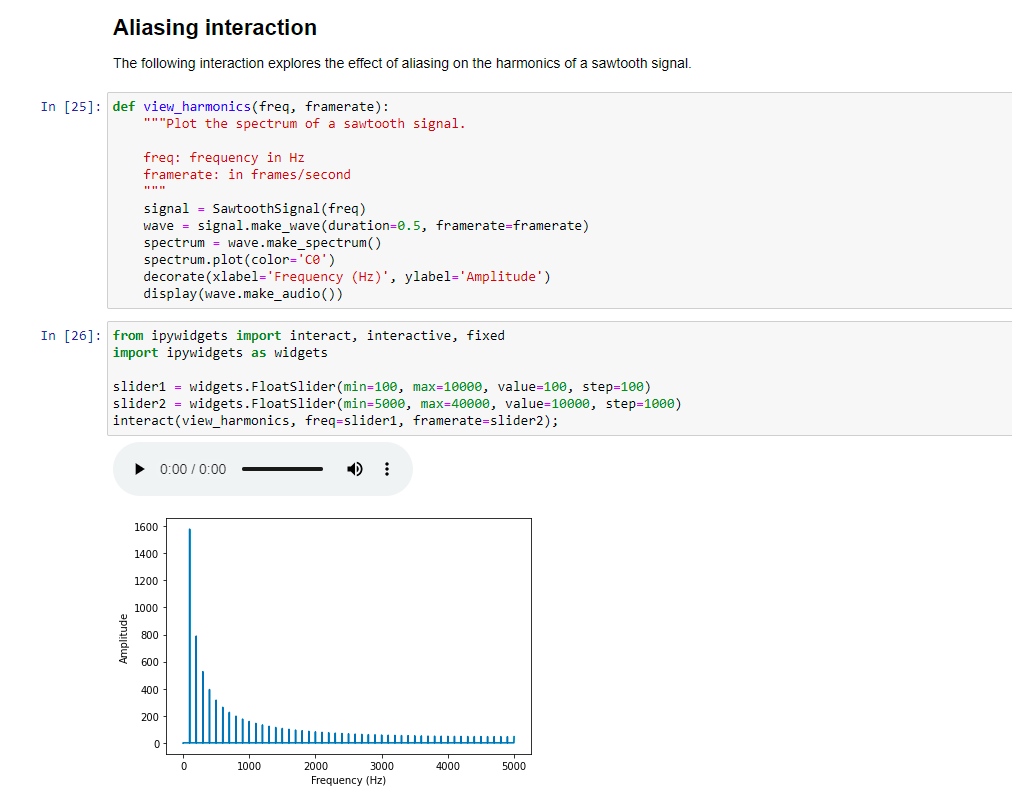
\includegraphics[width=\textwidth]{img/work_check.png}
            \caption{Everything is working fine}
            \label{fig:work_check}
        \end{figure}
    
    \newpage
        \section{Part 2: SawtoothSignal}

        In this part we need to create a \texttt{SawtoothSignal} class, that extends the \texttt{signal} class and provides an \texttt{evaluate} function. After it's done we can create its spectrum and compare it to the spectrum of triangle and square signals.
        
        Firstly we need to import required libraries to the project (Listing \ref{lst:sawtooth_def})
            
        \begin{lstlisting}[language=Python,caption={Sawrooth class definition},label={lst:sawtooth_def}]
    from thinkdsp import *
    import numpy as np
    
    class SawtoothSignal(Sinusoid):
        def evaluate(self, ts):
            graph = self.freq * ts + self.offset / np.pi / 2
            
            cutoff, _ = np.modf(graph) # create a cutoff
            ys = normalize(unbias(cutoff), self.amp)
            return ys
        \end{lstlisting}
        
        Next, we can check is our class works correctly (Listing \ref{lst:sawtooth_check}, Figure \ref{fig:sawtooth_wave_plot}).
            
        \begin{lstlisting}[language=Python,caption=Sawtooth wave plot code,label={lst:sawtooth_check}]
    sawtooth = SawtoothSignal()
    sawtooth_wave = sawtooth.make_wave(sawtooth.period * 3, framerate=40000)
    sawtooth_wave.plot()
    decorate(xlabel='Time (s)')
        \end{lstlisting}

        \begin{figure}[H]
          \centering
          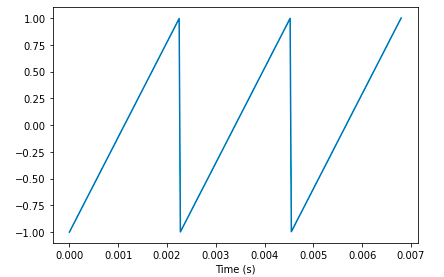
\includegraphics[width=\textwidth]{img/sawtooth_wave.png}
          \caption{Sawtooth's wave's plot}
          \label{fig:sawtooth_wave_plot}
        \end{figure}
            
        Next, spectrum of the created signal was created (Listing \ref{lst:sawtooth_spec}, Figure \ref{fig:sawtooth_spec}).
            
        \begin{lstlisting}[language=Python,caption=Sawtooth's spectrum computation,label={lst:sawtooth_spec}]
    sawtooth_wave.make_spectrum().plot()
    decorate(xlabel='Frequency (Hz)')
        \end{lstlisting}
        
        \begin{figure}[H]
          \centering
          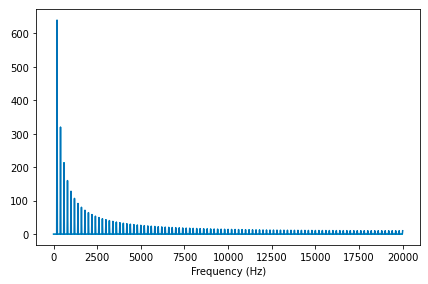
\includegraphics[width=\textwidth]{img/sawtooth_spec.png}
          \caption{Sawtooth's spectrum}
          \label{fig:sawtooth_spec}
        \end{figure}

        Compared to the triangle signal's spectrum and square signal's spectrum (Listring \ref{lst:spec_cmp}, Figure \ref{fig:sawtooth_cmp}), our sawtooth signal has spikes both on even and odd base frequencies factors, and it decreases linearly from its frequency.
            
        \begin{lstlisting}[language=Python,caption=Spectrum comparison code,label={lst:spec_cmp}]
    SquareSignal(200).make_wave(duration=0.5, framerate=10000).make_spectrum().plot(color='green')
    decorate(xlabel='Frequency (Hz)')
    TriangleSignal(200).make_wave(duration=0.5, framerate=10000).make_spectrum().plot(color='red')
    decorate(xlabel='Frequency (Hz)')
    sawtooth_wave.make_spectrum().plot(color='blue')
    decorate(xlabel='Frequency (Hz)')
        \end{lstlisting}    
            
        \begin{figure}[H]
            \centering
            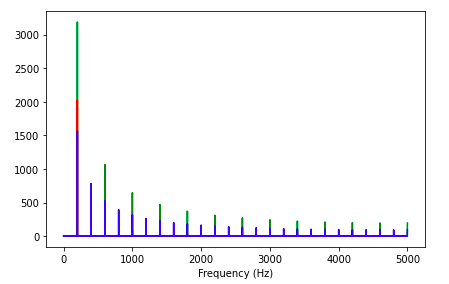
\includegraphics[width=\textwidth]{img/sawtooth_cmp.png}
            \caption{Spectrum comparison}
            \label{fig:sawtooth_cmp}
        \end{figure}
        
    \newpage
        \section{Part 3: Aliasing effect}
            
        In this part we need to explore the aliasing effect. 
        
        To reproduce this effect let's create a wave of frequency 1100 Hz and framerate of 10000 Hz (Listing \ref{lst:als_sqr}, Figure \ref{fig:als_sqr}). To comparison, this how this signal looks next to the signal with same frequency, but with framerate of 96000 Hz (Figure \ref{fig:als_clr}).
        
        
            
        \begin{lstlisting}[language=Python,caption=Waves creation,label={lst:als_sqr}]
    wave = SquareSignal(1100).make_wave(duration=9.6, framerate=10000)
    wave_clear = SquareSignal(1100).make_wave(duration=1, framerate=96000)
    wave.make_spectrum().plot(color='red')
    wave_clear.make_spectrum().plot(color='blue')
        \end{lstlisting}
            
        \begin{figure}[H]
            \centering
            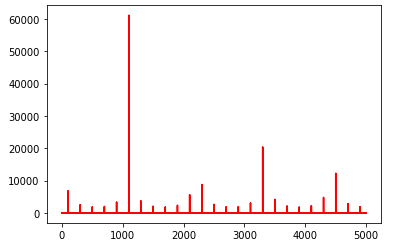
\includegraphics[width=\textwidth]{img/als_bad.png}
            \caption{Aliasing effect}
            \label{fig:als_sqr}
        \end{figure}
        
        \begin{figure}[H]
            \centering
            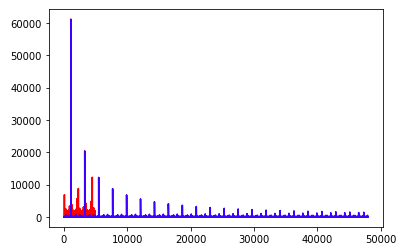
\includegraphics[width=\textwidth]{img/als_clear.png}
            \caption{Aliasing effect comparison}
            \label{fig:als_clr}
        \end{figure}
            
        By listening them, we can clearly notice the differenct: aliased signal is more "dirty" and "noisy".
            
    \newpage
        \section{Part 4: Spectrum's HS}
        
            In this part we need to explore, what is the HS values of the spectrum.
            
            To do it, let's create triangle signal with frequency of 440 Hz, length of the signal doesn't matter. Next, let's set its hs[0] = 100 and check, what is the deference.
            
            Code of this part - Listing \ref{lst:part4}
            
            \begin{lstlisting}[language=Python,caption=HS operations,label={lst:part4}]
                wave = TriangleSignal(440).make_wave(duration= 10 / 440, framerate=48000)
                spect = wave.make_spectrum()
                print(spect.hs[0])
                spect.hs[0] = 100
                print(spect.hs[0])
                spect_w = spect.make_wave()
                spect_w.normalize()
                spect_w.plot(color='red')
                wave.plot(color='blue')
            \end{lstlisting}
            
            \texttt{Spectrum.hs[0]=(-9.126033262418787e-14+0j)}, amplitude is a length, angle is a phase.
            
            As we can see, the is no difference between those signals (Figure \ref{fig:part4})
            
            \begin{figure}[H]
                \centering
                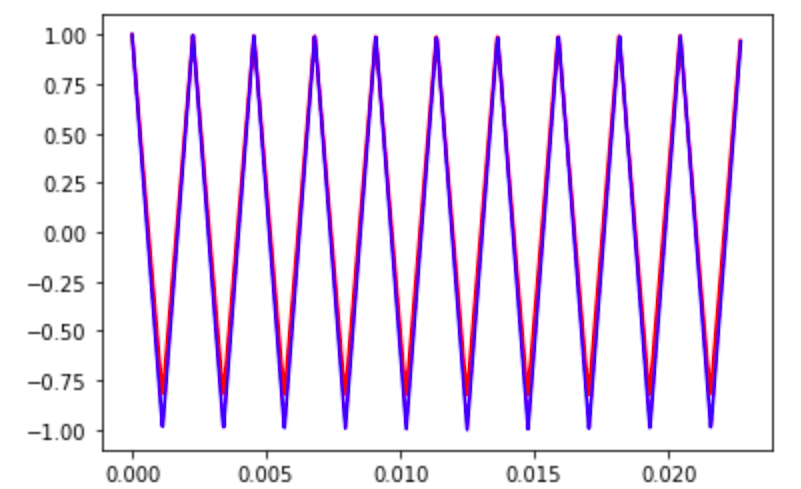
\includegraphics[width=\textwidth]{img/triag_no_diff.png}
                \caption{Function call result}
                \label{fig:part4}
            \end{figure}
            
    \newpage
        \section{Part 5: Muffling the signal}
        
            In this part we need to create a function, to muffle high frequencies of the wave by dividing hs by the frequency.
            
            Code of this part - Listing \ref{lst:part5_1}
            
            \begin{lstlisting}[language=Python,caption=Definition of the function,label={lst:part5_1}]
    def spectrum_muffle(spectrum):
        spectrum.hs[0] = 0
        spectrum.hs[1:] /= spectrum.fs[1:]
        return spectrum
            \end{lstlisting}
            
            Code of plotting: Listing \ref{lst:part5_2}.
            
            \begin{lstlisting}[language=Python,caption=Function usage,label={lst:part5_2}]
    wave = TriangleSignal(100).make_wave(duration=1, framerate=10000)
    spec = wave.make_spectrum()
    spec.plot(color='red', high=2000)
    spectrum_muffle(spec)
    spec.scale(100)
    spec.plot(color='blue', high=2000)
    decorate(xlabel='Frequency (Hz)')
            \end{lstlisting}
            
            As we can see, high frequencies are muffled (Figure \ref{fig:part5_2}). After listening we can be sure in it.
            
            \begin{figure}[H]
                \centering
                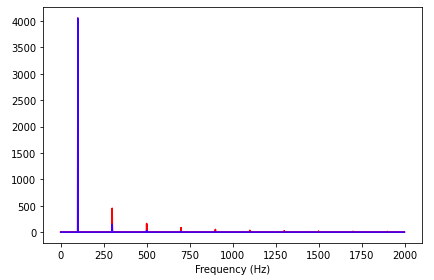
\includegraphics[width=\textwidth]{img/spec_muffle.png}
                \caption{Function call result}
                \label{fig:part5_1}
            \end{figure}
            
    \newpage
        \section{Part 6: New signal}
        
            In this part we need to find a signal, which similar to sawtooth signal, but its amplitude decreases by $1/f^2$ instead of $1/f$/.
            
            We can use sawtooth signal as base, and simply divide it's amplitudes by frequencies once more using function, declared in the previous part. Code is next: Listing \ref{lst:part6}. Result is next: Figure \ref{fig:part6}. We need to use such big framerate because of aliasing effect.
            
            \begin{lstlisting}[language=Python,caption=Signal and spectrum creation,label={lst:part5_1}]
s = SawtoothSignal(200).make_wave(duration=1, framerate=1000000).make_spectrum()
spectrum_muffle(s).plot(high = 5000)
            \end{lstlisting}
            
            \begin{figure}[H]
                \centering
                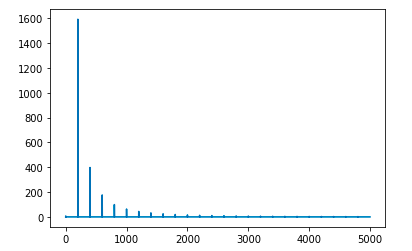
\includegraphics[width=\textwidth]{img/spec_f2.png}
                \caption{Spectrum of the signal}
                \label{fig:part5_1}
            \end{figure}
    
    \newpage
        \section{Conclusion}
            More advanced skills and knowledge of signals, waves and spectrum was acquired. Three more default signal types - triangle, square and sawtooth signals, which has specific features. Aliasing effect was explored. It has a lot of effect on decomposing the signal into the set of sine signals, that's why we need to have a higher framerate to not loss the data. Spectrum components was learned and used to muffle the signal.
            
            
    
\end{document}
